This reader contains the complete derivations of the whole adelic
prime-boundary complex, its equivariant comparison with the
Connes--Consani coefficient sheaf, and the continuous separation of all
endpoint extensions of the original zeta quotient. The actual source
distinction between primitive \(Z_1/\tau\) and the parity-bearing
integer \(1\) is retained by the explicit closed coefficient copies.
Primitive \(\tau\) is not assigned addition, parity, a numerical
coordinate, or a weight.

The active target remains the requested Deligne lifting theorem for the
full \(\tau\) programme. The calculations below prove global
endpoint-extension vanishing and the entire displayed comparison
triangle. They do not prove the remaining numerical purity statement or
RH. In particular the non-endpoint supported quotient is retained: the
separation polynomial is invertible on it, and cannot be called zero
there.

The complete user definitions, arguments and corrections are retained in
the private corpus. GAP0 and GEX0 identify the exact argument records
consulted and the receiving domains of every operation. The
user-originating global reconstruction argument is not replaced by an
assumption that a restricted receiving test space is the whole source
geometry.

The human constructions used here are Alain Connes's adelic
periodization; Alain Connes, Caterina Consani and Matilde Marcolli's
adelic Weil programme; Alain Connes and Caterina Consani's original
two-chart sheaf; Ralf Meyer's original spectral-function spaces; and
Pierre Deligne's local invariant-cycle and weight arguments. Exact
source versions, proof locators, prior programme credit and original
factors are given in the proofs that follow. A local source-reading
ledger distinguishes author TeX from the retained French transcription
of Deligne.

The complete arguments appear in this order: GAP, the entire global
comparison; GER, the original analytic inverse and all endpoint
corrections; GEX, the unique section and full extension groups; FDB, an
independent calculation of all prime degrees and signs; CTF, an
independent derivation of the entire comparison triangle and its
faithful coefficient extension. Earlier proof dependencies are retained
in the same local repository, with their original sources and version
records. Nothing in this reader is a remote-publication receipt.

\newpage

\begin{figure}
\centering
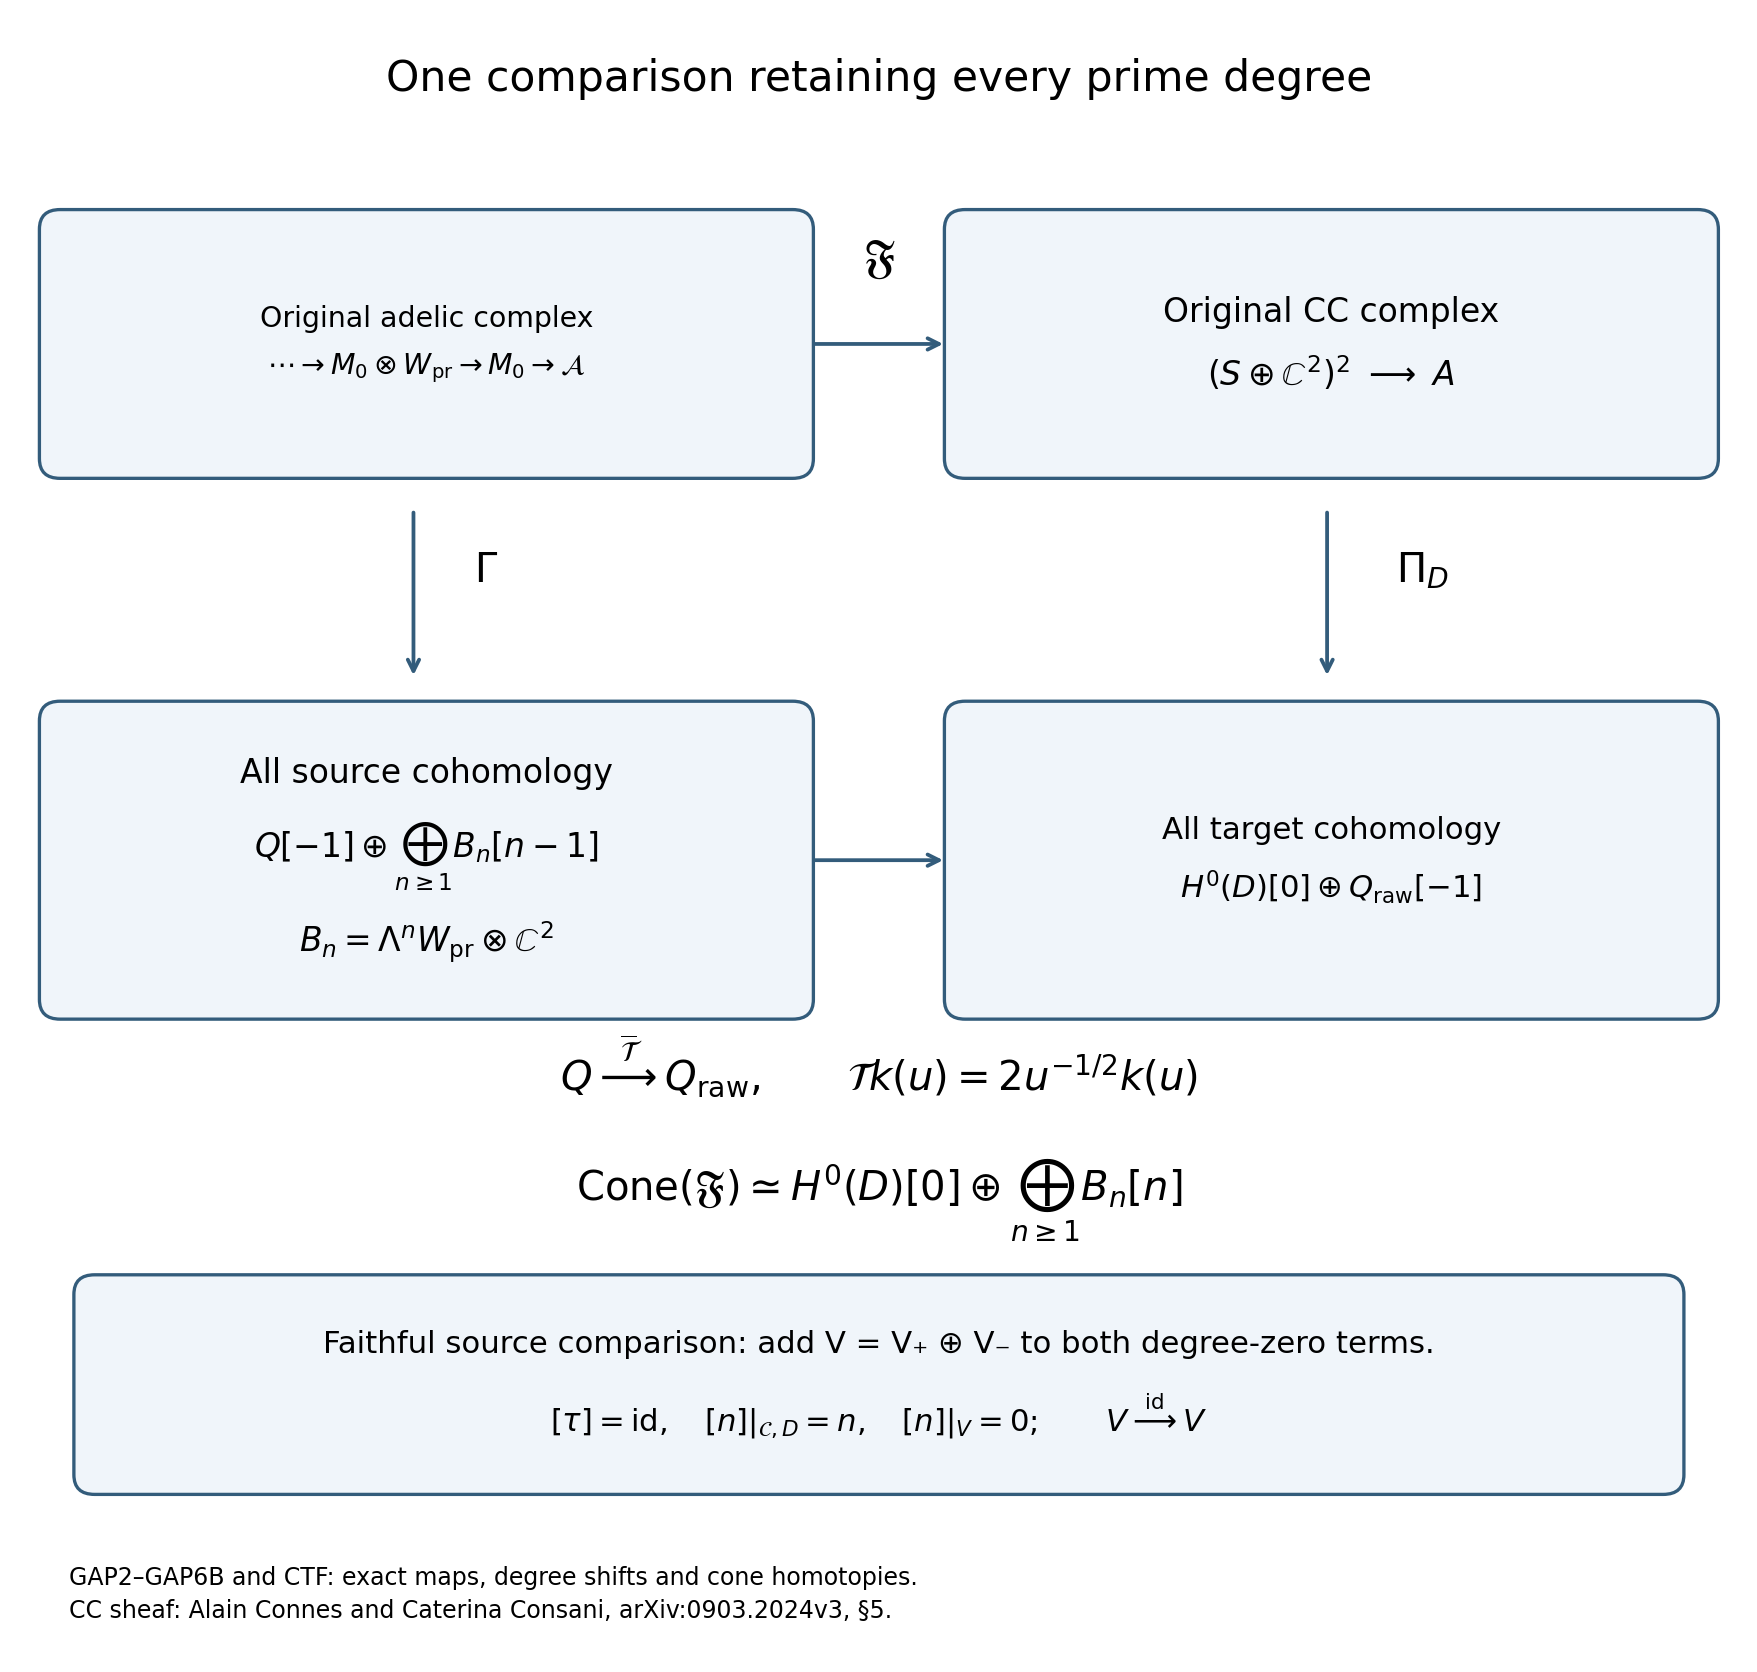
\includegraphics[width=\textwidth,height=.83\textheight,keepaspectratio]{tau_lifting_weights_20260924/GLOBAL_PRIME_COMPARISON.png}
\caption{The complete comparison, with all prime-boundary degrees}
\end{figure}

Figure 1. GAP2--GAP6B construct all objects and maps, including the full
ordered-prime exterior terms, the cohomology projections, Fourier
orientation and the faithful closed coefficient copies. The extra
identity-cone is retained and explicitly contracted. This diagram is
about constructed receiving complexes; it does not assign a vector
structure to primitive \(\tau\).

\newpage

\begin{figure}
\centering
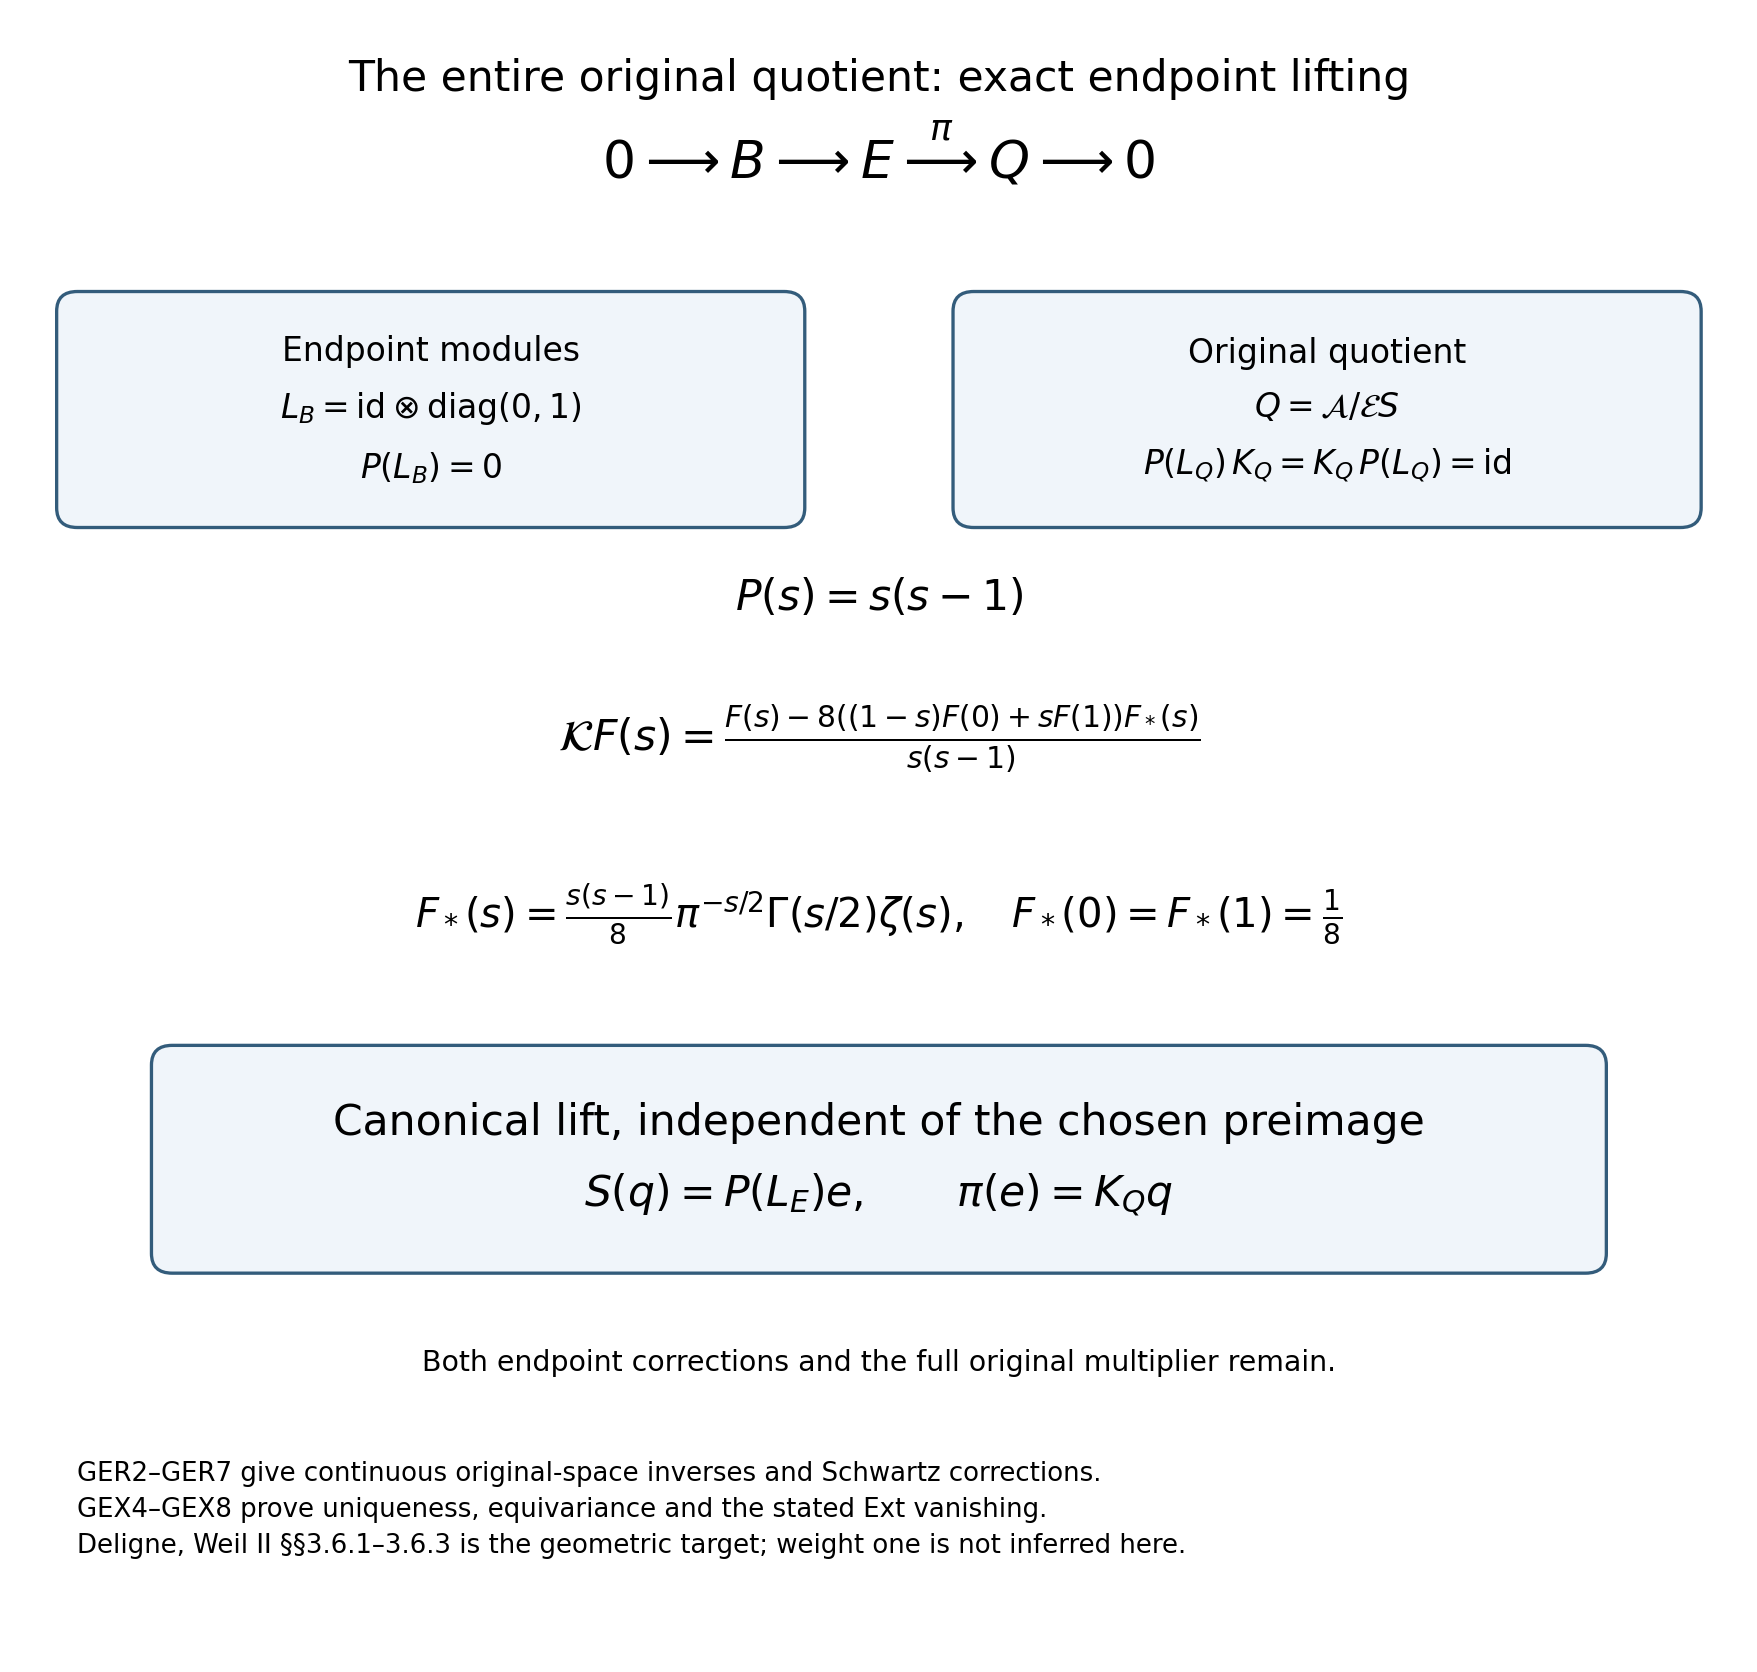
\includegraphics[width=\textwidth,height=.83\textheight,keepaspectratio]{tau_lifting_weights_20260924/GLOBAL_ENDPOINT_LIFT.png}
\caption{The exact global separation operator and lifting formula}
\end{figure}

Figure 2. GER2--GER7 construct the inverse on the actual original
quotient and its Schwartz return. GEX4--GEX8 prove the lift, its
continuity, full equivariance and all-degree extension vanishing in the
stated categories. The full original-zeta multiplier in the correction
is retained. DCP's different supported \(Q\)-term has the same
invertible polynomial action as the target; it is not an annihilated
endpoint module.
